%compile with pdflatex on papeeria

\documentclass[a4paper,12pt]{article}
\usepackage{fancyhdr}
%\usepackage{fancyheadings}
\usepackage[ngerman,german]{babel}
\usepackage{german}
\usepackage[utf8]{inputenc}
%\usepackage[latin1]{inputenc}
\usepackage[active]{srcltx}
%\usepackage{algorithm}
%\usepackage[noend]{algorithmic}
\usepackage{amsmath}
\usepackage{amssymb}
\usepackage{amsthm}
\usepackage{bbm}
\usepackage{enumerate}
\usepackage{graphicx}
\usepackage{ifthen}
\usepackage{listings}
\usepackage{enumitem}
%\usepackage{struktex}
\usepackage{hyperref}
\usepackage{tikz}
\usepackage{float}
\usepackage{subcaption}
\captionsetup{compatibility=false}
\captionsetup[subfigure]{labelformat=empty}

\usepackage{pgfplots}
\usepgfplotslibrary{fillbetween}
%\usetikzlibrary{patterns}
\pgfplotsset{compat=1.15}
\usepackage{mathrsfs}
\usetikzlibrary{arrows}

\pgfplotsset{grid style={dashed,gray}}

\definecolor{kolorwykresu}{rgb}{0.07,0.04,0.56}

\pagenumbering{gobble}

%%%%%%%%%%%%%%%%%%%%%%%%%%%%%%%%%%%%%%%%%%%%%%%%%%%%%%
%%%%%%%%%%%%%% EDIT THIS PART %%%%%%%%%%%%%%%%%%%%%%%%
%%%%%%%%%%%%%%%%%%%%%%%%%%%%%%%%%%%%%%%%%%%%%%%%%%%%%%
\newcommand{\Fach}{2. Klausur aus der Mathematik (A)}
\newcommand{\Name}{}
\newcommand{\datum}{}
\newcommand{\Matrikelnummer}{}
\newcommand{\Semester}{Q12/1}
\newcommand{\Uebungsblatt}{} %  <-- UPDATE ME
%%%%%%%%%%%%%%%%%%%%%%%%%%%%%%%%%%%%%%%%%%%%%%%%%%%%%%
%%%%%%%%%%%%%%%%%%%%%%%%%%%%%%%%%%%%%%%%%%%%%%%%%%%%%%

\setlength{\parindent}{0em}
\topmargin -1.0cm
\oddsidemargin 0cm
\evensidemargin 0cm
\setlength{\textheight}{9.2in}
\setlength{\textwidth}{6.0in}

%%%%%%%%%%%%%%%
%% Aufgaben-COMMAND
\newcommand{\Aufgabe}[1]{
  {
  \vspace*{0.5cm}
  \textsf{\textbf{Aufgabe #1}}
  \vspace*{0.2cm}
  
  }
}
%%%%%%%%%%%%%%
\hypersetup{
    pdftitle={\Fach{}: Übungsblatt \Uebungsblatt{}},
    pdfauthor={\Name},
    pdfborder={0 0 0}
}

\lstset{ %
language=java,
basicstyle=\footnotesize\tt,
showtabs=false,
tabsize=2,
captionpos=b,
breaklines=true,
extendedchars=true,
showstringspaces=false,
flexiblecolumns=true,
}

\title{Übungsblatt \Uebungsblatt{}}
\author{\Name{}}

\begin{document}
\thispagestyle{fancy}
%\lhead{\sf \large \Fach{} \\ %\small \Name{} - \Matrikelnummer{}
\lhead{\sf \large \Fach{} %\small \Name{} - \Matrikelnummer{}
}
\rhead{\sf \Semester{}   \datum{}}
%\rhead{\sf \Semester{} }
\vspace*{0.2cm}
%\begin{center}
%%\LARGE \sf \textbf{Übungsblatt \Uebungsblatt{}}
%\end{center}
%\vspace*{0.2cm}

%%%%%%%%%%%%%%%%%%%%%%%%%%%%%%%%%%%%%%%%%%%%%%%%%%%%%%
%% Insert your solutions here %%%%%%%%%%%%%%%%%%%%%%%%
%%%%%%%%%%%%%%%%%%%%%%%%%%%%%%%%%%%%%%%%%%%%%%%%%%%%%%

  Name: \underline{\hspace{7cm}}
%\draw[line width=1pt,color=ccqqqq,smooth,samples=100,domain=-6:7] plot(\x,{(1/12)*\x*\x+(1/3)*\x});
  \hfill
  Datum: \underline{\hspace{4cm}}

%\vspace{0,5cm}Die Rechenwege müssen nachvollziehbar sein!

\vspace{1,5cm} {TEIL A} - ohne Hilfsmittel. Bearbeitungszeit 35 min.
\vspace {0,2cm}
 

\Aufgabe{1: Analysis (7 BE)} 
Gegeben ist der Graph einer Funktion $f$(s. unten). Bestimmen Sie, ob die Aussagen wahr oder falsch sind. Begründen Sie jeweils Ihre Antwort. (F - Stammfunktion von f, f´ - Ableitungsfunktion von f)

\begin{enumerate}[label={\alph*)}]
  \item $F$ hat 3 Extrema
  \item $F$ hat 3 Wendepunkte
  \item $f'$ hat zwei Nullstellen
  \item $f'(1)=0$
  \item $f(2)=0$
  \item $f'(2)=0$
  \item $f'(-1)<0$
\end{enumerate}

\vspace{1cm}

\begin{center}
\begin{tikzpicture}[>=latex, x=2cm, y=2cm, line cap=round, line join=round, scale=1.5]
  \begin{axis}[
    unit vector ratio=1 1,
    axis x line=center,
    axis y line=center,
    %extra x tick style={tick style={very thick}}
    xtick={-3,-2,...,2,3},
    ytick={-2,-1,...,2,3},
    ticklabel style = {font=\scriptsize},
    ticklabel style={fill=white},
    %extra x ticks={0},
    %xticklabel style={anchor=south west},
    %minor x tick num=1,
    %minor y tick num=1,
    %minor tick num = 1,
    %x=1cm,    %größe der kästchen in x-richtung
    %y=1cm,    %größe der kästchen in y-richtung
    xlabel={$x$},
    ylabel={$y$},
    %grid=both,
    grid=major, grid style={gray!30},
    grid=minor, grid style={gray!30},
    ymajorgrids=true,
    xmajorgrids=true,
    %extra x ticks=0,
    extra x tick labels=$0$,
    extra x tick style={
     tick label style={
     anchor=north east}},
    xlabel style={above left},
    ylabel style={below right},
    axis line style = thick,
    xmin=-3.2,
    xmax=3.2,
    ymin=-2.2,
    ymax=3]
  
    \addplot[line width=1pt,color=kolorwykresu,smooth,samples=100, domain=-2.5:2.7]plot(\x,{0-(9/40)*((\x)+2)*((\x)-1)^(2)*((\x)-2)});
    \draw[color=kolorwykresu] (-2.2,-1.3) node[anchor=north west] {$f$};
  
  \end{axis}
  \end{tikzpicture}
\end{center}

% \begin{figure}[H]
% \centering
%   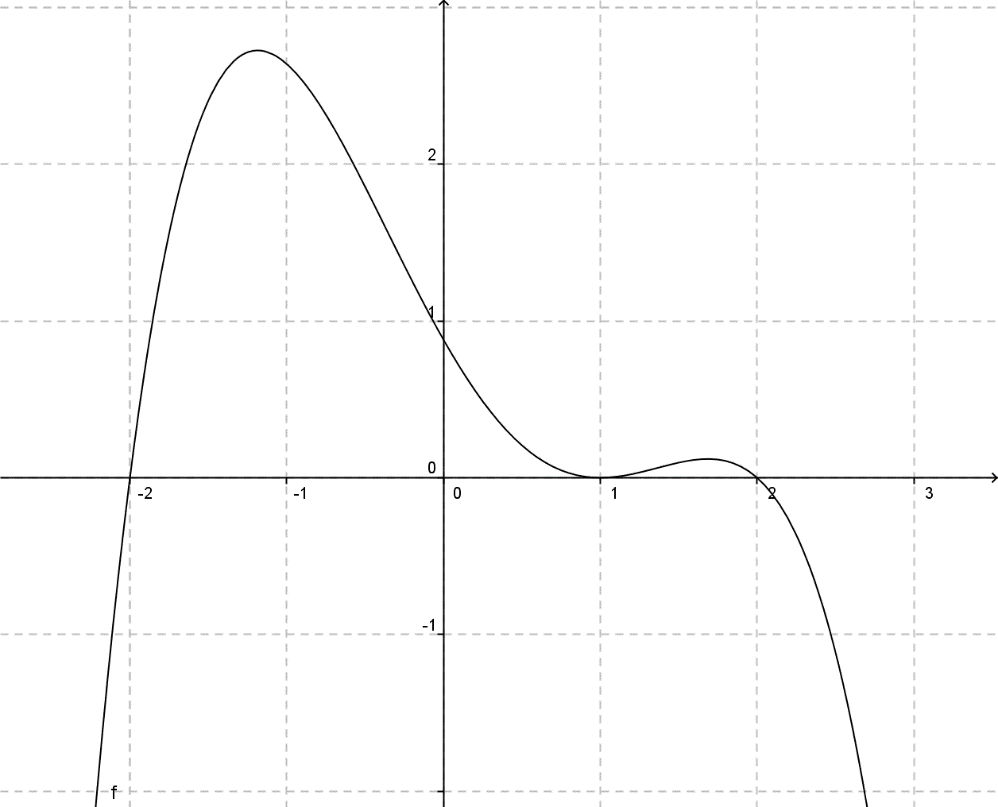
\includegraphics{210227.png}
% \end{figure}

\newpage
\vspace*{-4\baselineskip}


\Aufgabe{2: Stochastik (4 BE)}
Gegeben ist eine Zufallsgröße $X$, die die Werte $x_i = \{-2; 0; 2; 4\}$ annimmt.\\
Dem untenstehenden Histogramm kann man die Wahrscheinlichkeitswerte $P(X = x_i)$ entnehmen



\begin{figure}[h!]
  \centering
\begin{tikzpicture}[>=latex, line cap=round, line join=round,>=triangle 45, scale=1.8]

\begin{axis}[
  %unit vector ratio=1 10,
  axis x line=center,
  axis y line=center,
  axis line style = thick,
  xtick align=inside,
  xtick={-4,-2,0,2,4},
  ytick={0,0.1,0.2,0.3,0.4},
  xtick style=thick,
  ytick style=thick,
  xticklabels={,,},
  extra x ticks={-2,0,2,4},
  bar width=1cm,
  minor y tick num=9,
  x=1cm,    %größe der kästchen in x-richtung
  y=15cm,    %größe der kästchen in y-richtung
  xlabel={$x$},
  ylabel={$P(X=x)$},
  xmajorgrids=true,
  ymajorgrids=true,
  yminorgrids=true,
  minor grid style={gray!25},
  major grid style={black!50},
  xlabel style={below right},
  ylabel style={below right},
  xmin=-4,
  xmax=5,
  ymin=0,
  ymax=0.4]
  
  
\addplot[ybar,fill=blue,fill opacity=0.2] coordinates {
        (-2,0.17)
        (0,0.33)
        (4,0.14)
    };
\end{axis}
\end{tikzpicture}
\end{figure}

%\begin{figure}[h!]
%  \centering
%  \includegraphics[width=0.5\columnwidth]{210227_barChart_p.png}
%\end{figure}

Ergänzen Sie den zu $x_i=2$ gehörenden Wahrscheinlichkeitswert im Histogramm und ermitteln Sie den Erwartungswert der Zufallsgröße.

\Aufgabe{3 Geometrie (4 BE)}

 Gegeben sind die Geraden $g$ und $h$ mit den  Parametern $t, \alpha, \mu  \in R$
\[
\begin {aligned}
   g: \vec{X}= \begin{pmatrix} 4 \\
                              2 \\
                                -1
                  \end{pmatrix}
           + \alpha \begin{pmatrix} 1 \\
                                t\\
                                2
                  \end{pmatrix}
\end {aligned}
\qquad
\qquad
\begin {aligned}
    h: \vec{X}= \begin{pmatrix} 1\\
                              1 \\
                                1
                  \end{pmatrix}
           + \mu \begin{pmatrix} 4t \\
                                1 \\
                                4
                  \end{pmatrix}
\end {aligned}
%\raisebox{-10mm}{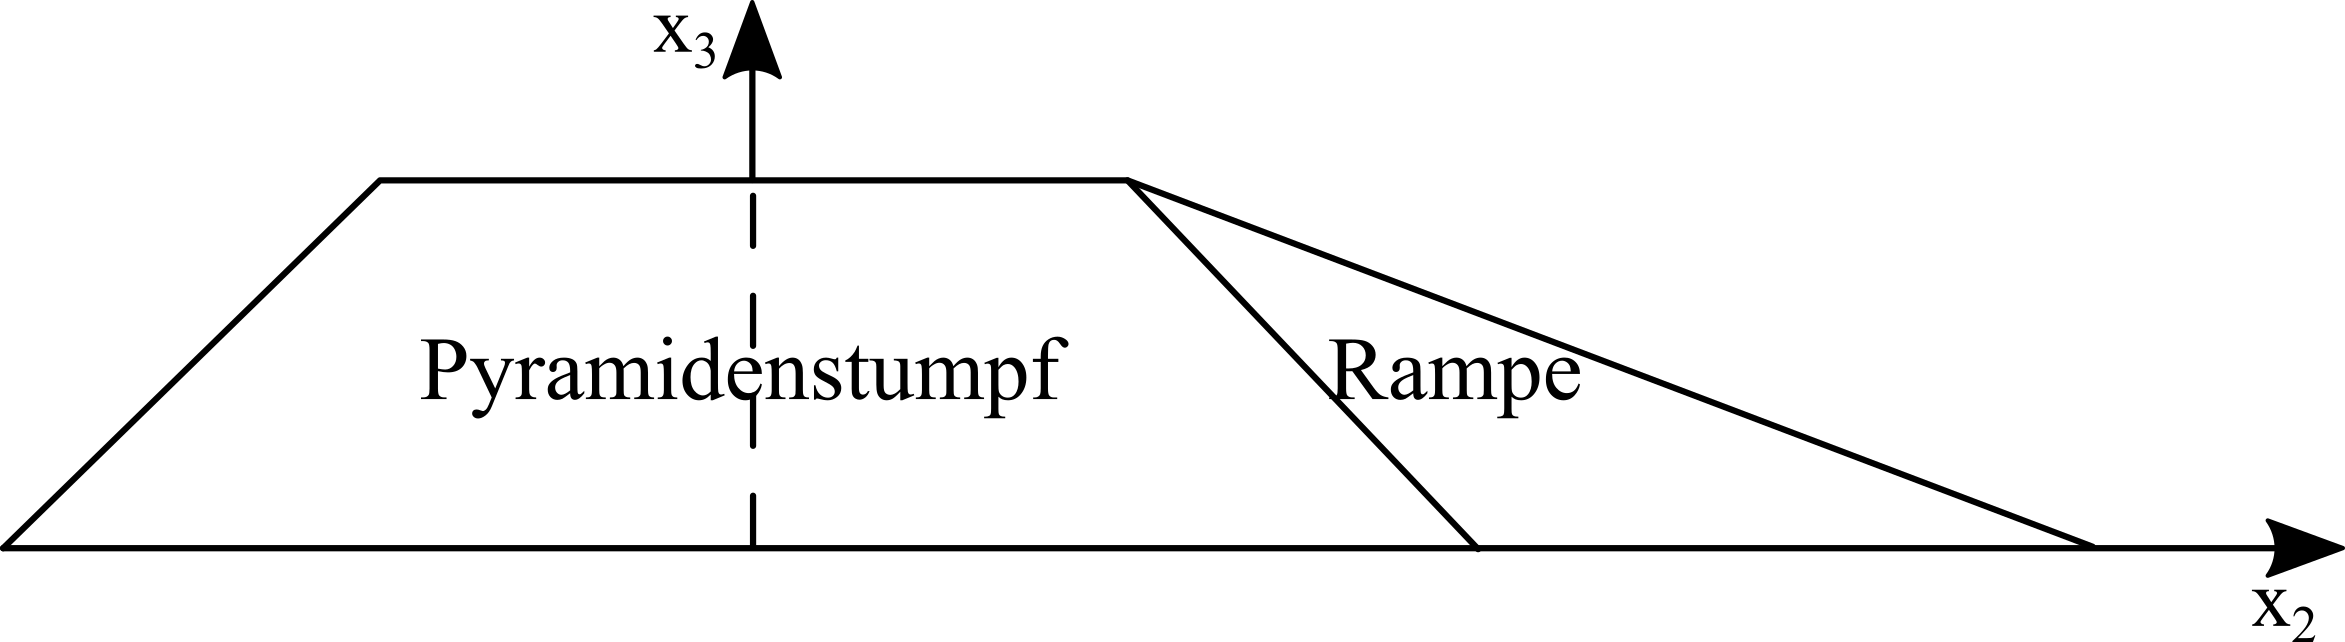
\includegraphics[keepaspectratio = true, scale = 0.5] {210227_pyramidenStumpfRampe.png}}
\]
\begin{enumerate}[label={\alph*)}] 
\item Bestimmen Sie den Parameter t so, dass die Geraden $g$ und $h$ zueinander parallel sind.
\item Belegen Sie dann, dass $g$ und $h$ nicht aufeinander liegen.
\end{enumerate}



\newpage
\vspace*{-4\baselineskip}
\enlargethispage{3cm}
{TEIL B} - mit Hilfsmittel. Bearbeitungszeit 100 min


\Aufgabe{4: Analysis (8 BE)}
Gegeben sei die Funktion $f: x\rightarrow x^3-6x^2+8x $.
Ihr Graph ist in der Abbildung dargestellt.\\

\begin{figure}[H]
  \centering

    \subfloat[]{

%\begin{tikzpicture}[>=latex, x=1cm, y=1cm, line cap=round, line join=round,>=triangle 45]
\begin{tikzpicture}[>=latex, x=2cm, y=2cm, line cap=round, line join=round, scale=1.7]
\begin{axis}[
  unit vector ratio=1 1,
  axis x line=center,
  axis y line=center,
  %extra x tick style={tick style={very thick}}
  xtick={-4,-2,...,4,6},
  ytick={-4,-2,...,3,4,6,8},
  ticklabel style = {font=\scriptsize},
  %,yshift=0.5ex},
  ticklabel style={fill=white},
  %extra x ticks={0},
  %xticklabel style={anchor=south west},
  %minor x tick num=1,
  %minor y tick num=1,
  %minor tick num = 1,
  %x=1cm,    %größe der kästchen in x-richtung
  %y=1cm,    %größe der kästchen in y-richtung
  xlabel={$x$},
  ylabel={$y$},
  %grid=both,
  grid=major, grid style={dashed,gray!30},
  grid=minor, grid style={dashed,gray!30},
  ymajorgrids=true,
  xmajorgrids=true,
  xlabel style={above left},
  ylabel style={below right},
  axis line style = thick,
  xmin=-4.5,
  xmax=8,
  ymin=-4.5,
  ymax=9]
%\coordinate (O) at (0,0)
%\addplot [mark=none,domain=-15:15] {};
% \draw[line width=1pt,color=ccqqqq,smooth,samples=100,domain=-15:65] plot(\x,{0.5*\x *e^(-0.1*\x+2)});
  %      \draw[line width=1pt,color=ccqqqq,smooth,samples=100,domain=-15:65] plot(\x,{50 *\x+2});
%    \draw[line width=2pt,color=qqwuqq,smooth,samples=100,domain=-21.518627341217258:25.46534828151831] plot(\x,{5*((\x)^(2)/3-(\x)^(3)/20)});
  %\addplot[line width=1pt,color=ccqqqq, domain=-15:65]plot(\x,{0.5*\x*e^(-0.1*\x+2)});
  \addplot[line width=1pt,color=kolorwykresu,smooth,samples=100, domain=-5:10]plot(\x,{((\x)^(3)-6*(\x)^(2)+8*(\x))});
  \draw[color=kolorwykresu] (4.5,8.5) node[anchor=north west] {$G_f$};

\end{axis}
\end{tikzpicture}

        %\addplot[line width=1pt,color=ccqqqq ]plot(\x,{0.5*\x*e^(-0.1*\x+2)});

%\draw (26.07701146189816,9.323776772024983) node[anchor=north west] {G_f};
%\begin{scriptsize}
%\draw[color=ccqqqq] (0.06341005665314936,-6.095192074225563) node {$f$};
%\end{scriptsize}
%\end{axis}
%\end{tikzpicture}

    }

\end{figure}


\begin{enumerate}[label={\alph*)}]
\item Gegeben sind die Punkte $O(0|0)$, $N(2|0)$  und $M(4|0)$ . Weisen Sie nach, dass der Punkt $N$ der Wendepunkt von f ist und ermitteln Sie die Gleichung der Wendetangente $ w$ im Punkt N. 
\item Die Wendetangente $ w$, die y-Achse und die Funktion $f$ schließen zwischen den Punkten O und N ein Flächenstück ein. Bestimmen Sie dessen Flächeninhalt und markieren Sie das Flächenstück in der obigen Abbildung.

\end{enumerate}

\Aufgabe{5: Analysis (8 BE)}

Ein Computervirus wird auf die Rechner dieser Welt losgelassen. Der Virus breitet sich erst
aus und wird dann bekämpft. Die Funktion $v (t )=3 t e^{-t}$
beschreibt modellhaft, wie viele
Millionen Rechner vom Virus befallen sind. t gibt die Zeit ab dem Ausbruch in Tagen an.
\begin{enumerate}[label={\alph*)}]
\item Berechnen Sie, an welchem Tag die meisten Rechner betroffen waren und wie viele waren das.
\item Berechnen Sie, an welchem Tag der Rückgang der Anzahl der befallenen Computer am stärksten war.
\item  Begründen Sie, wie sich der Virusbefall auf lange Sicht entwickeln wird.
\end{enumerate}

\newpage
\vspace*{-3\baselineskip}


\Aufgabe{6: Stochastik (11 BE)}
Beim Spielen mit einem Würfel stellt der Stefan fest, dass die Augenzahl 1 überdurchschnittlich häufig, die Augenzahl 6 dagegen relativ selten auftritt. Diese führt zu der Vermutung, dass der Würfel gezinkt ist und die Wahrscheinlichkeit eine 6 zu würfeln, nur $10\%$ beträgt. Gehen Sie zunächst davon aus, dass die Vermutung zutrifft.
Mit dem Würfel wird 100-mal nacheinander gewürfelt. Die Zufallsgröße X zählt die Anzahl der Sechsen.
\begin{enumerate}[label={\alph*)}]


\item Berechnen Sie mithilfe von Bernoulli Formel  die Wahrscheinlichkeit, dass in 100 Würfen genau 10 Sechsen auftreten.
\item Berechnen Sie die Wahrscheinlichkeit, dass in 100 Würfen mindestens 16 Sechsen auftreten.
\item Berechnen Sie Erwartungswert $\mu$ und Standardabweichung $\sigma$ und bestimmen Sie die Wahrscheinlichkeit, dass X um höchstens $1,5 \sigma$ von $ \mu$ abweicht.\\
\\
\\
Mit dem Würfel wird mehrmals nacheinander gewürfelt.
\item Ermitteln Sie, wie oft ein Spieler mindestens würfeln muss, um einer Wahrscheinlichkeit von wenigsten 95\% mindestens einmal eine 6 zu erhalten.
\item Bestimmen Sie die Wahrscheinlichkeit, dass erst im fünften Wurf zum ersten Mal eine Sechs auftritt.
\end{enumerate}

\vspace{10cm} 
\begin{flushright}bitte wenden \end{flushright}


\newpage
\vspace*{-4\baselineskip}

\enlargethispage{1,5cm}
\Aufgabe{7: Geometrie (12 BE)}
Eine ägyptische Pyramide hat die Form einer geraden quadratischen Pyramide. Die Seitenlänge des Grundquadrats beträgt 160m, die Höhe der Pyramide 100m. Im Modell in einem Koordinatensystem mit Längeneinheit 1m liegt der Ursprung genau in der Mitte der quadratischen Grundfläche und die $x_1$- und $x_2$-Achse verlaufen parallel zu den Grundkanten. 

  \begin{figure}[H]
    \centering
    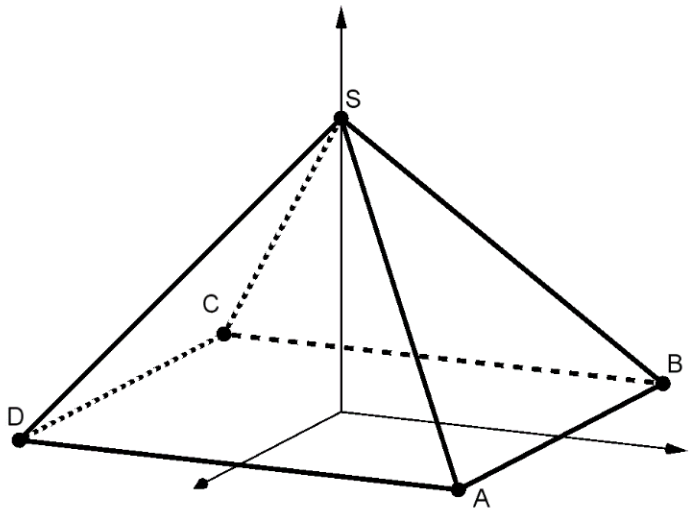
\includegraphics[width=0.5\columnwidth]{210227_pyramide.png}
    %\caption{A boat.}
    %\label{fig:boat1}
  \end{figure}




\begin{enumerate}[label={\alph*)}]
  \item Geben Sie die Koordinaten der Eckpunkte $A$,$B$ und $S$ an und bestimmen Sie die Gleichung der Ebene $E$ durch diese Punkte in Koordinatenform.\\
    {\it [mögliches Teilergebnis: $E: 5x_2 + 4x_3 = 400$]}
  \item Die Ägypter bauten die Pyramide schichtweise. Zum Transport der Steine zur jeweiligen Schicht wurde eine Rampe benötigt. Die Rampe führt entlang der Geraden\\

\[
\begin {aligned}
    r: \vec{X}= \begin{pmatrix} 0 \\
                              200 \\
                                0
                  \end{pmatrix}
           + \mu \begin{pmatrix} 0 \\
                                24 \\
                                -5
                  \end{pmatrix}
\end {aligned}
\qquad
\qquad
\raisebox{-10mm}{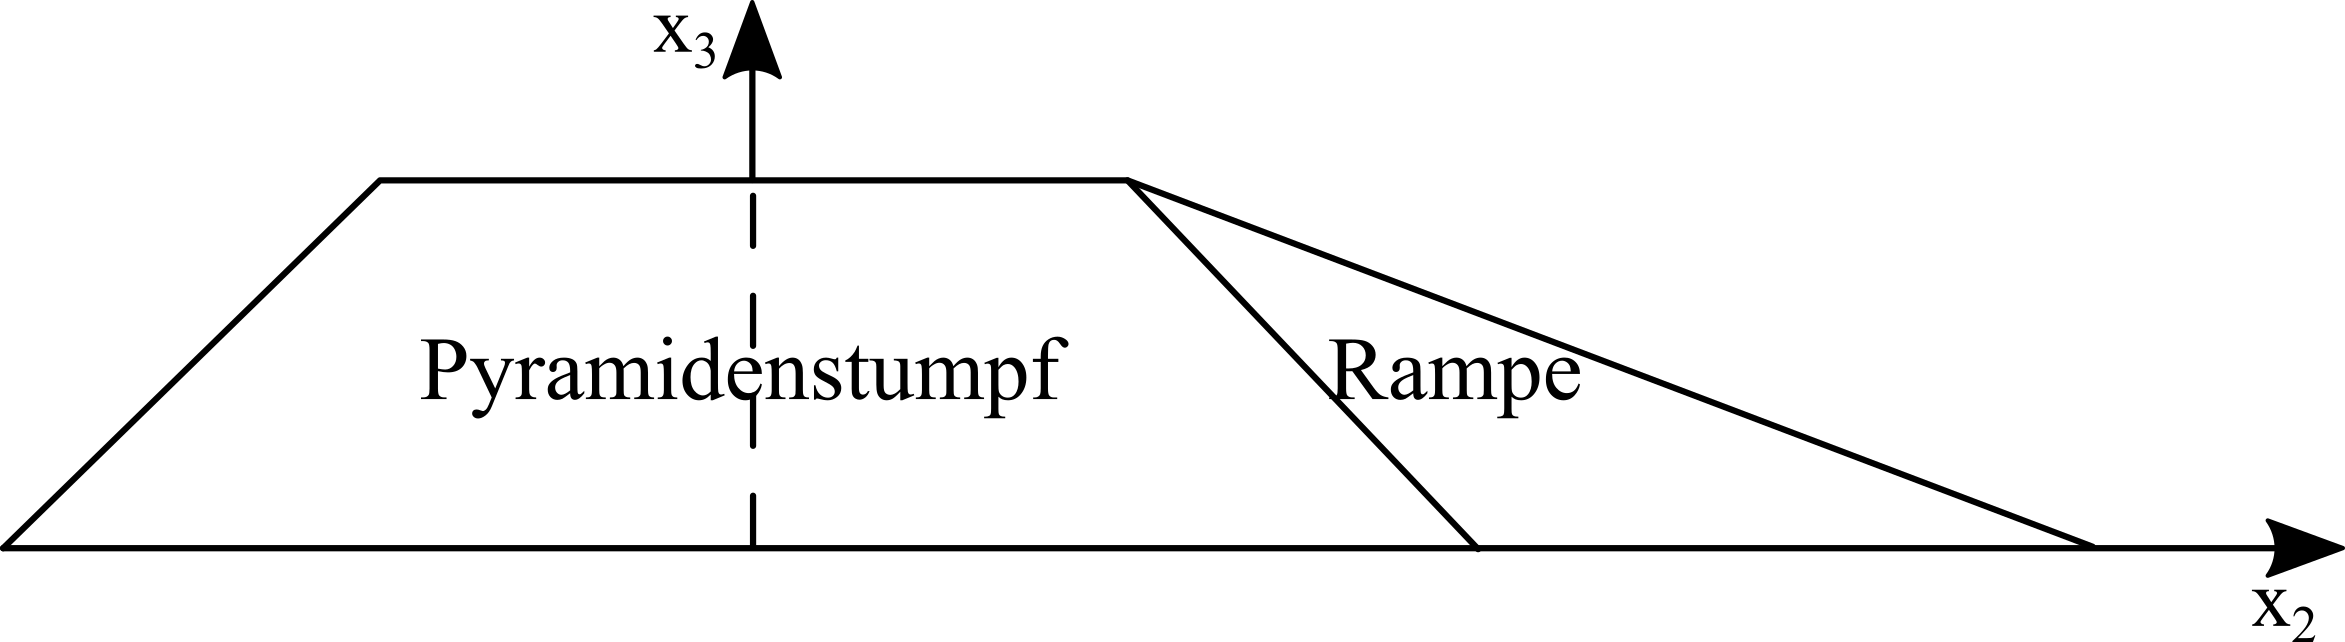
\includegraphics[keepaspectratio = true, scale = 0.5] {210227_pyramidenStumpfRampe.png}}
\]


  vom Erdboden bis an den Rand des bisher errichteten Pyramidenstumpfs und liegt in der $x_2 x_3$ Ebene.\\
    
    Berechnen Sie die Höhe des bisher gebauten Pyramidenstumpfes und die Länge der Rampe.\\

  \item  Der Punkt T$(0|60|25)$ liegt auf der Seitenfläche $ABS$. Er ist der Einstiegspunkt zu einem Schacht, der senkrecht zu dieser Seitenfläche verläuft und in 13m Höhe über der Grundfläche am Eingang der inneren Grabkammer endet. Berechnen Sie die Koordinaten dieses Endpunkts.
\end{enumerate}



\centerline{Viel Erfolg}


%\enlargethispage{2\baselineskip}

%\addtolength{\voffset}{-2cm}




%\begin{tikzpicture}
%\draw [very thin, black, step=0.5cm] (0,0) grid +(15,18);
%\end{tikzpicture}




%%%%%%%%%%%%%%%%%%%%%%%%%%%%%%%%%%%%%%%%%%%%%%%%%%%%%%
%%%%%%%%%%%%%%%%%%%%%%%%%%%%%%%%%%%%%%%%%%%%%%%%%%%%%%
\end{document}
